\chapter{质心 刚体}

\section*{A 组}
\vspace{0.3cm}
\textbf{5-1} 用质量线密度为 $\lambda$ 常量的细丝构成如图所示的无限内接等边三角形框架, 最外层的等边三角形 $ABC$ 的每边长为 $a$ , 而后在其三边中点内接各边长为 $a / 2$ 的等边三角形, 再在上方各边长为 $a / 2$ 的等边三角形三边中点内接边长为 $a / 4$ 的等边三角形……

(1) 试求框架的总质量 $m$;

(2) 确定框架质心 $C_{0}$ 与顶点 $A$ 之间的距离 $h$.


\begin{center}
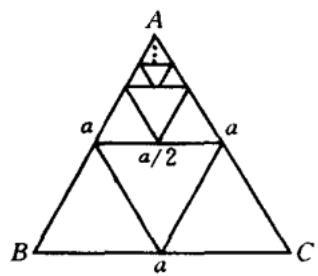
\includegraphics[width=0.2\textwidth]{figures/图5_1.jpg}
\end{center}

\vfill

\textbf{5-2} 质量线密度相同,但长度未必相同的三根细棒若能构成一个三角形,试确定此三角形框架的质心位置.

\vfill

\newpage

\textbf{5-3} 习题1-29中,人的质量设为 $M$ ,每个小球的质量同设为 $m$ ,取较长的抛球游戏时间,试求地面对人的平均支持力 $\overline{N}$ .


\vfill

\textbf{5-4} 系统如图, 两小球 $A$, $B$ 质量相同, 轻绳一半在水平桌面外, $A$ 球与桌面间无摩擦. 将 $B$ 球从静止自由释放后, 试问在 $A$ 球尚未离开桌面前 $B$ 球能否已碰到桌子侧面？

\begin{center}
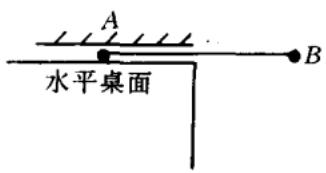
\includegraphics[width=0.2\textwidth]{figures/图5_4.jpg}
\end{center}

\vfill

\newpage

\textbf{5-5} 系统和有关参量均如图所示, 开始时两个物块都处于静止状态, 轻弹簧压缩量为 $l$. 设水平地面光滑, 试求撤去右侧外压力后, 系统质心可获得的最大加速度值 $a_{C0}$ 和最大速度值 $v_{C0}$ .

\begin{center}
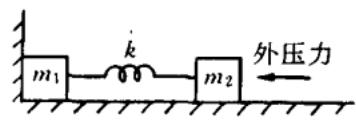
\includegraphics[width=0.2\textwidth]{figures/图5_5.jpg}
\end{center}

\vfill

\textbf{5-6} 各边长为 $a$、质量为 $M$ 的匀质刚性正方形细框架，开始时静止在光滑水平桌面上，框架右侧边中央有一小孔 $P$，桌面上另有一个质量为 $m$ 的小球以初速 $v_{0}$ 从小孔 $P$ 外射入. 设 $v_{0}$ 的方向如图所示, 小球与框架碰撞无摩擦且为弹性.

(1) 证明小球仍能从小孔 $P$ 射出框架；

(2) 计算小球从射入到射出小孔全过程的时间及它相对于桌面的平均速度.

\begin{center}
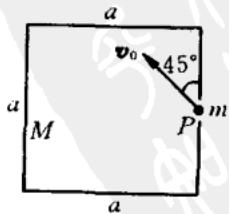
\includegraphics[width=0.2\textwidth]{figures/图5_6.jpg}
\end{center}

\vfill

\newpage

\textbf{5-7} 两个滑冰运动员质量都是 $m$ ，在两条相距 $l_0$ 的光滑平直冰道上均以 $v_0$ 速率相向匀速滑行。当他们之间的距离等于 $l_0$ 时，分别抓住一根长 $l_0$ 的轻绳两端，而后每人都用力缓慢往自己一边拉绳子，直到两者相距 $l$ 为止。计算这一过程中两人拉力所作总功 $W$ ，进而确认 $W$ 等于系统动能增量 $\Delta E_k$ 。

\vfill

\textbf{5-8} 质量分别为 $m_{1}, m_{2}$ 的两个质点构成的系统，试证在其质心系中的动能为 $\frac{1}{2} \mu \Delta v \cdot \Delta v$ ，式中 $\mu$ 为两质点的约化质量， $\Delta v$ 为两质点的相对速度。

\vfill

\newpage

\textbf{5-9} 内外半径几乎同为 $R$ 、质量为 $M$ 的匀质圆环，静止地平放在水平桌面上，环内某直径的两端各有一个质量同为 $m$ 的静止小球。今以一个恒定的水平力 $\pmb{F}$ 拉环， $\pmb{F}$ 方向线通过环心且与上述直径垂直，如图所示。设系统处处无摩擦，试求两小球相碰前瞬间的相对速度大小 $v$ 。

\begin{center}
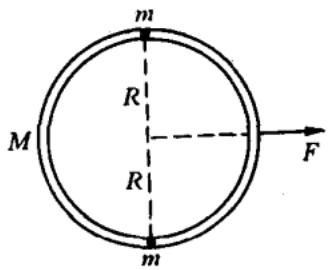
\includegraphics[width=0.2\textwidth]{figures/图5_7.jpg}
\end{center}

\vfill

\textbf{5-10} 两个质量相同的小球 $A, B$ ，用长为 $2a$ 的轻绳联结，开始时 $A, B$ 位于同一竖直线上， $B$ 在 $A$ 的下方，相距为 $a$ ，如图所示。今给 $A$ 水平初速度 $\pmb{v}_0$ ，同时静止释放 $B$ ，不计空气阻力，且设绳一旦伸直便不再回缩。试问经多长时间 $t, A, B$ 恰好第一次位于同一水平线上？

\begin{center}
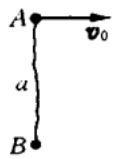
\includegraphics[width=0.2\textwidth]{figures/图5_9.jpg}
\end{center}

\vfill

\newpage

\textbf{5-11} 已知质量 $m$、半径 $R$ 的匀质薄球壳相对直径轴的转动惯量为 $\frac{2}{3}mR^{2}$ ，试求质量 $m$，内、外半径分别为 $R_{2}, R_{1}$ 的匀质球壳相对直径轴的转动惯量 $I$.

\vfill

\textbf{5-12} 图所示的钟摆, 由质量 $m$、长 $l$ 的匀质细杆和质量 $M$、半径 $R$ 的匀质圆盘连接而成, 试求相对于过摆端 $A$ 并且与摆面垂直的轴的转动惯量 $I_{A}$ .

\begin{center}
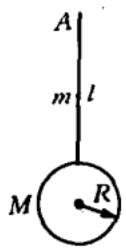
\includegraphics[width=0.1\textwidth]{figures/图5_11.jpg}
\end{center}

\vfill

\newpage

\textbf{5-13} 质量 $m$ 的匀质细丝, 在平面上弯曲成两个半径同为 $R$ 的相切连接的半圆形状, 如图所示. 过左半圆周中点 $A$ 设置垂直于圆平面的转轴, 试求弯曲细丝相对此转轴的转动惯量 $I_{A}$ .

\begin{center}
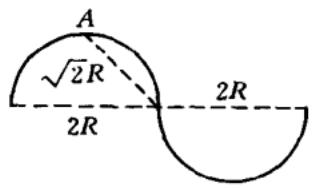
\includegraphics[width=0.2\textwidth]{figures/图5_12.jpg}
\end{center}

\vfill

\textbf{5-14} 两根质量同为 $m$、长度同为 $l$ 的匀质细杆，对称地联结成丁字尺，如图所示。过尺上每一点部位设置垂直于尺平面的转轴，转动惯量记为 $I$，试求 $I_{min}$ 和 $I_{max}$ 。

\begin{center}
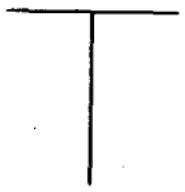
\includegraphics[width=0.2\textwidth]{figures/图5_14.jpg}
\end{center}

\vfill

\newpage

\textbf{5-15} 在图 5-15 所示的薄平板刚体中， $P_{1}$ 和 $P_{2}$ 两点相距 2l， $P_{2}$ 和 $P_{3}$ 两点相距 $l$， $P_{3}$ 和 $P_{1}$ 两点相距 $\sqrt{3}l$ 。已知刚体绕通过 $P_{1}$ 点的垂直轴的转动惯量为 $I_{1}=I_{C}+ml^{2}$ ，绕通过 $P_{2}$ 点的垂直轴的转动惯量为 $I_{2}=I_{C}+3ml^{2}$ ，其中 $I_{C}$ 为刚体绕通过质心 $C$ 的垂直轴的转动惯量。设 $I_{C}, m, l$ 已知，试求刚体绕通过 $P_{3}$ 点的垂直轴的转动惯量 $I_{3}$ 。

\begin{center}
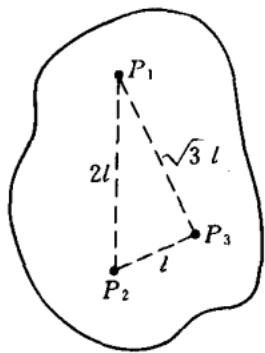
\includegraphics[width=0.2\textwidth]{figures/图_5_15.jpg}
\end{center}

\vfill

\textbf{5-16} 匀质正方形薄板质量为 $m$、各边长为 $a$，如图所示，在板平面上设置过中心 $O$ 的转轴 MN，求板相对该轴的转动惯量 $I$.

\begin{center}
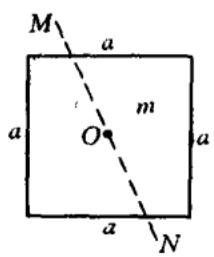
\includegraphics[width=0.2\textwidth]{figures/图5_17.jpg}
\end{center}

\vfill

\newpage

\textbf{5-17} 系统和参量如图所示, 物块与水平桌面间无摩擦, 轻绳与实心匀质滑轮间无相对滑动, 滑轮与转轴间无摩擦, 试求物块运动加速度 $a$.

\begin{center}
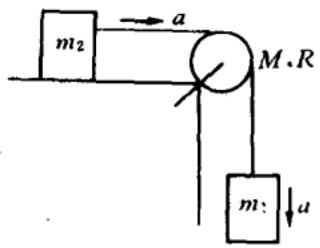
\includegraphics[width=0.2\textwidth]{figures/图5_19.jpg}
\end{center}

\vfill

\textbf{5-18} 两个匀质圆盘质量分别为 $m_{1}, m_{2}$ ，半径分别为 $R_{1}, R_{2}$ ，各自可绕互相平行的固定水平轴无摩擦地转动，轻皮带紧围在两个圆盘外侧，如图所示。今对圆盘1相对其转轴施加外力矩 $M$ ，圆盘、皮带都被带动，设圆盘、皮带间无相对滑动，试求圆盘1,2各自的转动角加速度 $\beta_{1}, \beta_{2}$ 。

\begin{center}
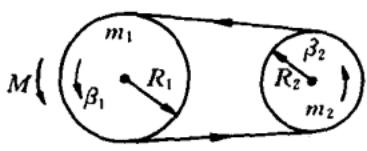
\includegraphics[width=0.3\textwidth]{figures/图_5_20.jpg}
\end{center}

\vfill

\newpage

\textbf{5-19} 某竖直平面内有一半径为 $R$ 的固定半圆环，它的两个端点等高. 如图所示, 质量 $m$、长 $R$ 的匀质细杆一端靠着环的端点, 另一端在环内壁, 从静止自由滑下. 设杆与环内壁间无摩擦, 试求细杆滑到最低位置时两端各受环的支持力 $N_{1}, N_{2}$ .

\begin{center}
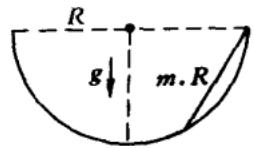
\includegraphics[width=0.2\textwidth]{figures/图5_21.jpg}
\end{center}

\vfill

\textbf{5-20} 某刚体可绕过其 $A$ 点的水平固定轴无摩擦地自由转动，开始时刚体静止地处于图5-22所示位置，它的质心 $C$ 到转轴的垂线恰好处于水平状态。刚体自由释放后，已知 $C$ 到达最低处时转轴对刚体的支持力是刚体重力的 $\alpha (\alpha > 1)$ 倍，试问过程中转轴提供的最大水平支持力是刚体重力的多少倍？

\begin{center}
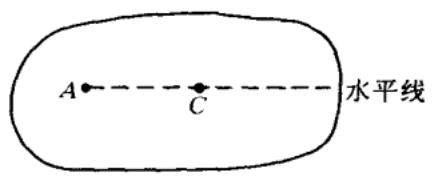
\includegraphics[width=0.3\textwidth]{figures/图5_22.jpg}
\end{center}

\vfill

\newpage

\textbf{5-21} 如图所示, 一颗小子弹水平射击静止悬挂于顶端 $A$ 的匀质长棒下端, 棒长为 $l$, 质量为 $M$. 设碰撞时间为 $\Delta t$ , 碰后瞬间棒绕 $A$ 端固定光滑水平转轴的角速度为 $\omega$ , 试求碰撞过程中转轴提供的水平方向平均支持力的方向和大小 $\overline{N}_{\parallel}$ .

\begin{center}
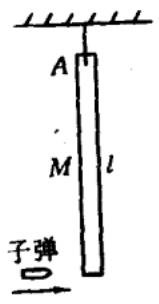
\includegraphics[width=0.1\textwidth]{figures/图5_24.jpg}
\end{center}

\vfill

\textbf{5-22} 长度为 2(长度取某约定单位)的刚性细杆 AB，两端被约束在 $y=x^{2}$ 的固定抛物线轨道上运动。当 AB 杆恰好与 $x$ 轴平行时，$A$ 端的速度大小为 $v_{A}$ ，试确定此时 AB 杆中点 $P$ 的速度大小 $v_{P}$ 。

\vfill

\newpage

\textbf{5-23} 半径为 $R$ 、质量为 $m$ 的匀质球体静止于倾角为 $\phi$ 的斜面上， $t = 0$ 开始纯滚下来，试求在滚到斜面底部前的 $t$ 时刻瞬心 $M$ 的加速度 $a_{M}$ 。再问，球体与斜面间的摩擦因数 $\mu$ 为多大？


\vfill

\textbf{5-24} 半径为 $r$、质量为 $m$ 的匀质轮子，以角速度 $\omega_{0}$ 旋转。现将轮子轻轻地放在水平地面上，轮与地面间的摩擦因数设为处处相同。

(1) 求运动稳定后轮子的动量大小及对轮心的角动量大小；

(2) 由功的定义式直接计算过程中摩擦力所作总功, 验证此功等于轮子动能增加量.

\vfill

\newpage

\textbf{5-25} 如图所示, 质量 $m$ 的平板受水平力 $F$ 的作用沿水平地面运动, 板与地面间的摩擦因数为 $\mu$ . 板上放一质量为 $M$、半径为 $R$ 的匀质圆柱体, 圆柱体与板间的摩擦因数也为 $\mu$ .

(1) 若圆柱体在板上的运动是纯滚动, 求板的加速度;

(2) 为使圆柱体在板上仍作纯滚动, 试求 $F$ 可取的最大值.

\begin{center}
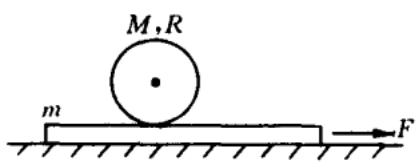
\includegraphics[width=0.3\textwidth]{figures/图5_29.jpg}
\end{center}

\vfill

\textbf{5-26} 如图所示, 在倾角为 $\theta$ 的固定斜面上, 一质量为 $m$ 、半径为 $r$ 的匀质圆柱体上绕有轻绳, 绳的另一端缠绕在斜面顶端的定滑轮上, 定滑轮是质量 $M$ 、半径 $r$ 的匀质圆盘. 设圆柱体沿斜面滚下时细绳拉直且不能伸长, 并与斜面平行, 细绳与圆柱体及定滑轮之间无相对滑动, 略去滑轮轴承处的摩擦.

(1) 若圆柱体的运动为纯滚动, 求其质心加速度;

(2) 试求圆柱体作纯滚动的条件.

\begin{center}
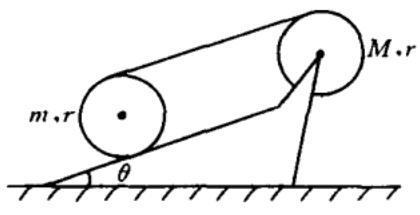
\includegraphics[width=0.3\textwidth]{figures/图5_31.jpg}
\end{center}


\vfill

\newpage

\textbf{5-27} 有两个相同的匀质球体 $A, B$ ，开始时 $B$ 球静止在水平地面上， $A$ 球在此地面上朝着 $B$ 球作匀速纯滚动， $A, B$ 随即发生弹性碰撞。碰后 $A, B$ 因与地面间有摩擦，最后都达到稳定的匀速纯滚状态，试求全过程中系统动能损失百分比 $\alpha$ 。


\vfill

\textbf{5-28} 质量 $M$ 、长 $L$ 的匀质细杆 $AB$ , 某时刻在水平桌面上绕着它的中心 $C$ 以角速度 $\omega$ 逆时针方向旋转, 同时 $C$ 又具有与杆垂直的水平向右速度 $v_{C}$ , 如图所示. 设细杆各部位与桌面间的摩擦因数同为 $\mu$ , 试求该时刻 $C$ 的加速度方向和大小 $a_{C}$ 以及细杆的角加速度方向和大小 $\beta$ .

\begin{center}
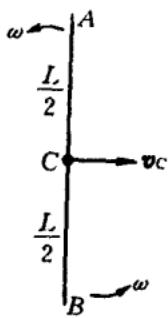
\includegraphics[width=0.1\textwidth]{figures/图5_33.jpg}
\end{center}


\vfill

\newpage

\textbf{5-29} 匀质细杆 $AB$ ，开始时静止地靠墙竖立在水平地面上，后因轻微扰动而倾斜滑动。设系统处处无摩擦，试问当图5-35中倾角 $\phi$ 达何值时杆的 $A$ 端将离墙？

\begin{center}
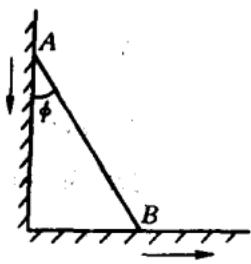
\includegraphics[width=0.2\textwidth]{figures/图5_35.jpg}
\end{center}


\vfill

\textbf{5-30} 光滑水平桌面上静放一根匀质细杆,一小球在桌面上以垂直于细杆长度方向的速度朝着细杆 $P$ 部位运动,如图所示.设两者发生弹性碰撞,试求碰后小球与 $P$ 间分离速度大小与碰前两者接近速度大小的比值.

\begin{center}
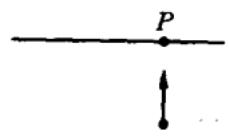
\includegraphics[width=0.25\textwidth]{figures/图_5_37.jpg}
\end{center}


\vfill

\newpage

\textbf{5-31} 如图所示, 匀质细杆 AB 静放在光滑水平桌面上,小球 $P$ 在此平面上对准杆的 $B$ 端运动, 速度方向与杆的长度方向垂直. 已知球与细杆弹性碰撞后, 两者又会发生第二次碰撞, 试求杆的质量与球的质量比 $\gamma$ .

\begin{center}
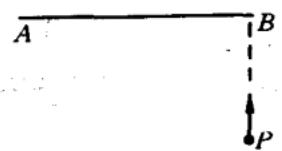
\includegraphics[width=0.25\textwidth]{figures/图5_39.jpg}
\end{center}

\vfill

\textbf{5-32} 在长为 $l$ 的轻轴一端装上回转仪的轮子, 轴的另一端吊在长为 $L$ 的绳上. 当轮子绕轴快速转动且轴处于水平状态时, 轮子将绕着过支点 $O$ 的竖直轴进动, 如图所示. 已知轮子质量为 $m$ , 相对于自转轴的转动惯量为 $I_0$ , 自转角速度为 $\omega_s$ , 轮子质心位于中心, 试求绳与竖直线之间的小夹角 $\beta$ .


\begin{center}
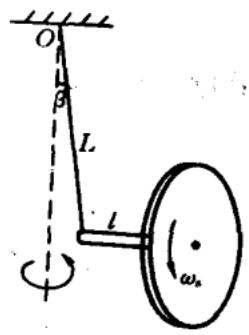
\includegraphics[width=0.2\textwidth]{figures/图_5_41.jpg}
\end{center}

\vfill

\newpage

\textbf{5-33} 如图所示, 用夹子去夹半径 $R$ 的对称球体. 已知夹子两臂与球表面间的静摩擦因数为 $\mu$ , 若球可以不动, 略去重力, 试求图中线度 $l$.

\begin{center}
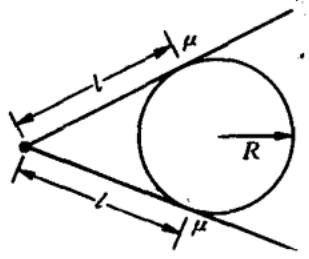
\includegraphics[width=0.2\textwidth]{figures/图5_42.jpg}
\end{center}

\vfill

\section*{B 组}
\vspace{0.3cm}
\textbf{5-34} 试用物理方法证明任意三角形三条边上的高共点.

\vfill

\newpage

\textbf{5-35} 如图所示, 质量 $m$ 的对称滑板装置 $A$ 开始时静止在倾角为 $\phi$ 的斜面上， $A$ 的底板长 $L$ ，底部与斜面之间的摩擦因数 $\mu < \frac{1}{2} \tan \phi$ . 今在 $A$ 的底板上方正中间静止放一个质量也是 $m$ 的小滑块 $B$ ，两者之间光滑接触. 将 $A, B$ 同时释放后， $A, B$ 分别向下滑动， $A$ 的前部挡板还会与 $B$ 发生弹性碰撞. 设斜面足够长，试求从开始释放到 $A$, $B$ 发生第 3 次碰撞间

(1) 经历过的时间 $T$;

(2) 摩擦力所作功 $W_{f}$ .


\begin{center}
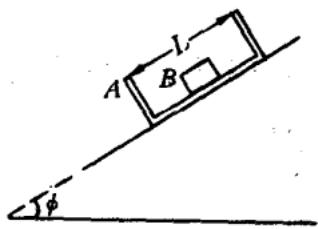
\includegraphics[width=0.2\textwidth]{figures/图5_45.jpg}
\end{center}

\vfill

\textbf{5-36} 轻质细杆两端分别固定小球 $A, B$ . $B$ 球的质量是 $A$ 球质量的 $\alpha$ 倍, 其中 $\alpha > 1$ . 开始时细杆左半部分静止在水平桌面上, 右半部分露在桌面外. 自由释放后, 细杆会绕着桌面侧棱倾斜偏转, 即图5-46中的 $\phi$ 角会从零增大. 开始时, 倾斜偏转过程中细杆中点一直不离开桌面侧棱, 直到倾角 $\phi$ 达到某 $\phi_0 (0 < \phi_0 < \pi / 2)$ 值时, 细杆中点开始滑离桌面侧棱, 试求细杆中部与桌面侧棱之间的摩擦因数 $\mu$ .

\begin{center}
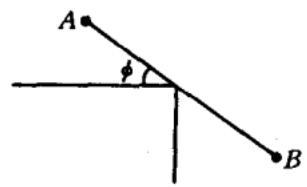
\includegraphics[width=0.2\textwidth]{figures/图5_46.jpg}
\end{center}

\vfill

\newpage

\textbf{5-37} 动能为 $E_{0}$ 的 ${}^{4}He$ 核轰击静止的 ${}^{7}Li$ 核，作完全非弹性碰撞后成为复合核 ${}^{11}B$ ，后者进一步分裂成 ${}^{10}B$ 和中子 ${}^{1}n$ 。上述核反应过程需消耗能量 $\theta=2.8MeV$ ，反应方程为
\[
{ } ^ { 4 } \mathrm{He} + { } ^ { 7 } \mathrm{Li} \longrightarrow ( { } ^ { 1 1 } \mathrm{B} ) \longrightarrow { } ^ { 1 0 } \mathrm{B} + { } ^ { 1 } \mathrm{n} - 2 . 8 \mathrm{MeV} ,
\]
试求上述核反应过程所需的 $E_{0}$ 最小值及对应的中子动能值.


\vfill

\textbf{5-38} 讨论地球在月球引力作用下的潮汐现象.

取地球和月球构成的系统, 地球中心 $O$ 绕着系统质心作圆周运动, 地心参考系为平动变速非惯性系. 在地心系中设置 Oxy 坐标系, 某时刻月球位于 $x$ 轴上, 月心的坐标 $x_{M}=r_{M}$ 中的 $r_{M}$ 即为地心与月心的间距. 设想地球表面被海水层覆盖, 潮汐作用使其表面相对地球半径 $R_{\mathrm{E}}$ 有起伏，如图所示。在Oxy平面上取一块质量为 $m$ 的海水，位于海水表面 $x, y$ 处。不考虑地球自转影响，试求：

(1) 该块海水所受潮汐力；

(2) 图中 $A$, $B$ 两处海水的高度差 $h_{AB}$ .

已知：月球质量 $M=7.35\times10^{22}$ kg, $r_{M}=3.84\times10^{8}$ $m$, $R_{E}=6.37\times10^{6}$ $m$.

\begin{center}
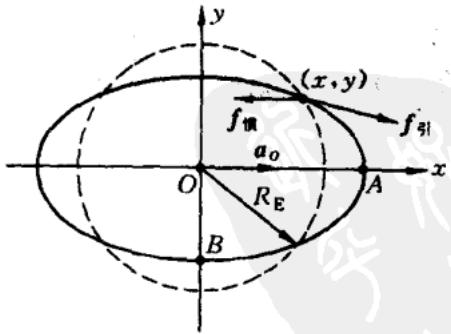
\includegraphics[width=0.3\textwidth]{figures/图_5_48.jpg}
\end{center}

\vfill

\newpage

\textbf{5-39} 如图所示, 匀质立方体的质量为 $m$ 、各边长为 $a$ , 试求该立方体绕对角线轴 MN 的转动惯量 $I$.


\vfill

\textbf{5-40} 椭圆细环的半长轴为 $a$ ，半短轴为 $b$ ，质量为 $m$ （未必匀质）。已知细环绕长轴的转动惯量为 $I_{a}$ ，试求细环绕短轴的转动惯量 $I_{b}$ 。

\vfill

\textbf{5-41} 如图所示, 质量为 $m$ 的匀质圆柱体, 截面半径为 $R$, 长为 2R, 试求圆柱体绕通过中心及两底面边缘转轴的转动惯量 $I$.

\begin{center}
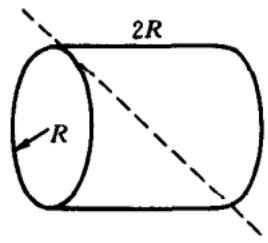
\includegraphics[width=0.2\textwidth]{figures/图5_51.jpg}
\end{center}

\vfill

\newpage

\textbf{5-42} 某人手握长棒一端猛击岩石, 意欲使棒折断. 为在碰撞时, 手不致于受到很大的冲击力, 设棒长 $L$ 且匀质. 试问碰撞点与手的距离 $l$ 取什么值较为合适?

\vfill

\textbf{5-43} 半径为 $R_{1}, R_{2}$ ，质量为 $m_{1}, m_{2}$的两个匀质圆盘，各自以角速度 $\omega_{1},\omega_{2}$ 绕自己的中心竖直轴顺时针方向无摩擦地在水平面上旋转.而后使它们缓慢移近，互相接触后保持转轴不动，如图所示.

(1) 计算两盘在接触处摩擦力作用下，各自最终的转动角速度 $\omega_{1}^{\prime}, \omega_{2}^{\prime}$ .

(2) 试问过程中在地面系中能否找到一个参考点 $P$，使得系统相对 $P$ 点角动量守恒？

\begin{center}
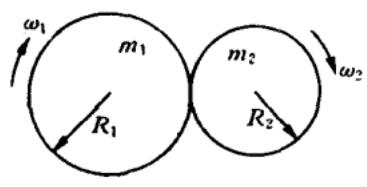
\includegraphics[width=0.3\textwidth]{figures/图5_54.jpg}
\end{center}

\vfill

\newpage

\textbf{5-44} 半径 $R$ 的均匀圆木在水平地面上以平动速度 $v_{0}$ 作匀速纯滚动时，与高 $h$ 的台阶相遇，接触处发生完全非弹性碰撞，即在碰撞后图5-56中圆木与台阶侧棱接触部位 $A$ 的速度降为零.再设两者间的摩擦因数足够大，使得部位 $A$ 不会与台阶侧棱在而后的接触过程中发生相对滑动.

(1) $v_{0}$ 和 $h$ 取何值时, 圆木能绕侧棱滚上台阶;

(2) 在(1)问基础上, 确定部位 $A$ 与侧棱间摩擦因数 $\mu$ 的取值范围.

\begin{center}
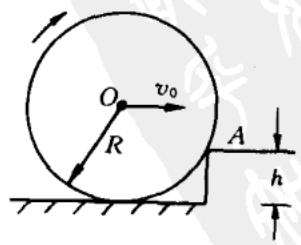
\includegraphics[width=0.3\textwidth]{figures/图_5_56.jpg}
\end{center}

\vfill

\textbf{5-45} 刚体在参考系 $S$ 中作平面平行运动时, 不同时刻的瞬心在 $S$ 系中的位置可形成迹线 $L$ . $t$ 时刻刚体瞬心 $M$ 在 $L$ 上的位置可用 $S$ 系中的位矢 $\mathbf{R}_M$ 标记, $\mathbf{R}_M$ 是随时间 $t$ 变化的矢量. 引入 $\pmb{v}_M^* = \mathrm{d}\pmb{R}_M / \mathrm{d}t$ , 称为刚体瞬心在迹线上的转移速度, 再将刚体在 $S$ 系中的转动角速度记为 $\omega$ , 试导出刚体瞬心加速度 $\pmb{a}_M$ 与 $\pmb{v}_M^*$ , $\omega$ 的关系, 且给出两个实例.

\vfill

\newpage

\textbf{5-46} 在光滑水平地面上有一质量 $M$ 、半径 $R$ 的匀质圆盘，盘边缘有一质量为 $m$ 的小车（处理成质点），开始时系统静止，而后小车沿盘边缘逆时针方向运动，如图所示。若小车相对圆盘转过 $N$ 圈，试问小车与盘心连线相对地面逆时针方向还是顺时针方向转过多少圈？

\begin{center}
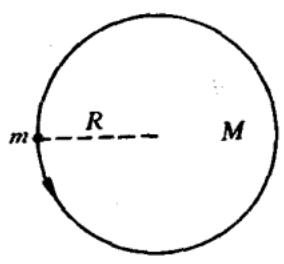
\includegraphics[width=0.2\textwidth]{figures/图5_61.jpg}
\end{center}

\vfill

\textbf{5-47} 半径 $R$、质量 $m$ 的匀质球壳，开始时以角速度 $\omega_{0}$ 绕水平直径轴旋转. t=0 时将球壳无初始平动地轻放在水平地面上，球壳与地面间的摩擦因数为 $\mu$ .

(1) 确定球壳恰好达到纯滚状态的时刻 $t_{0}$ ;

(2) 确定 $0 \leqslant t < t_{0}$ 时刻瞬心的位置 $M$ 及其加速度 $a_{M}$ .

\vfill

\newpage

\textbf{5-48} 如图所示, 质量 $m$、半径 $R$ 的匀质圆环静止在水平地面上, 它的水平直径右端点连结一个质量也是 $m$ 的小物体 $P$. 系统自由释放后, 假设环与地面间不会发生相对滑动, 试求圆环转过 $\theta$ 角时,

(1) 圆环转动角速度 $\omega;$

(2) 圆环受地面静摩擦力 $f$.

\begin{center}
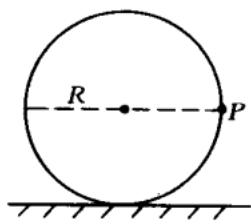
\includegraphics[width=0.2\textwidth]{figures/图5_65.jpg}
\end{center}

\vfill

\textbf{5-49} 质量 $m$ 、半径 $r$ 的匀质球位于倾角为 $\theta$ 的斜面底端。开始时球的中心速度为零，球相对过中心且与斜面平行的水平轴以角速度 $\omega_0$ 旋转，如图所示。已知球与斜面间的摩擦因数 $\mu > \tan \theta$ ，球在摩擦力作用下会沿斜面向上运动，试求球能上升的最大高度 $h$ 。

\begin{center}
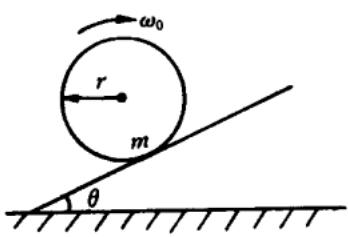
\includegraphics[width=0.2\textwidth]{figures/图5_67.jpg}
\end{center}

\vfill

\newpage

\textbf{5-50} 光滑桌面上有两个半径同为 $R$ 、质量同为 $m$ 的匀质刚性圆盘 $A, B$ . 设 $A$ 以平动速度 $\pmb{v}$ 与静止的 $B$ 相碰, 接触时连心线与 $\pmb{v}$方向线成 $45^{\circ}$ 夹角，如图所示.已知碰撞过程中连心线方向为弹性碰撞，但接触处有切向摩擦，摩擦因数为 $\mu$ 试求碰后 $A,B$ 的平动速度 $\pmb{v}_A,\pmb{v}_B$ 和各自转动角速度 $\omega_{A},\omega_{B}$ ，答案须按图中所示的 $x,y,z$ 坐标轴给出各矢量的分量表述

\begin{center}
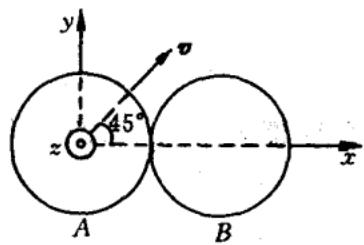
\includegraphics[width=0.3\textwidth]{figures/图_5_70.jpg}
\end{center}

\vfill

\textbf{5-51} 匀质细杆的 $A$ 端约束在光滑的水平长横梁上, 且可在横梁上自由滑行, 引入细杆与竖直方向夹角 $\theta$ 如图所示. 设开始时 $\theta = \pi / 2$ , 而后从静止释放细杆, 试问 $\theta$ 降到多大锐角时横梁给细杆 $A$ 端的向上支持力 $N$ 等于细杆所受重力 $mg$ ?

\begin{center}
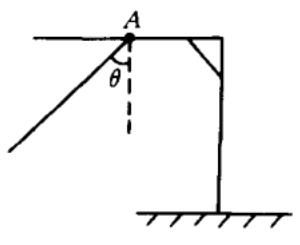
\includegraphics[width=0.2\textwidth]{figures/图_5_71.jpg}
\end{center}

\vfill

\newpage

\textbf{5-52} 如图所示, 质量 $M$ 的匀质细杆 AB 静止在光滑水平面上, $B$ 端的弹簧机构(其质量可略)将质量 $m$ 的小球相对地面以速度 $v$ 水平弹出, $v$ 的方向与 AB 杆的夹角记为 $\phi$ . 设弹出的小球恰好能与细杆的 $A$ 端相遇, 且细杆转过的角度不超过 $\pi$ , 试求质量比 $\gamma = M/m$ 和角度 $\phi$ 的取值范围.

\begin{center}
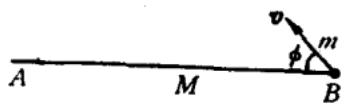
\includegraphics[width=0.2\textwidth]{figures/图5_73.jpg}
\end{center}

\vfill

\textbf{5-53} 如图 5-75 所示, 在匀质刚性圆盘中间切割出一个半径为原圆盘半径二分之一的同轴小圆盘, 切割使小圆盘与其外部圆环之间形成很小的缝隙, 缝隙宽度虽可略, 但它却使小圆盘与圆环之间只有点接触 (因盘有厚度, 实际上相接触的是垂直于盘面的一小段直线). 将系统放在水平地面上, 通过打击使它们具有共同的沿水平方向的速度 $v_{0}$ . 设圆环与地面间的摩擦因数 $\mu_{0} = 0.5$ , 圆环与小圆盘间的摩擦因数记为 $\mu$ .

(1) 设在而后的运动过程中, 圆环与小圆盘之间曾发生过相对滑动, 试确定 $\mu$ 的取值范围;

(2) 取 $\mu=0.2$ ，试求系统最后沿水平方向的速度。

\begin{center}
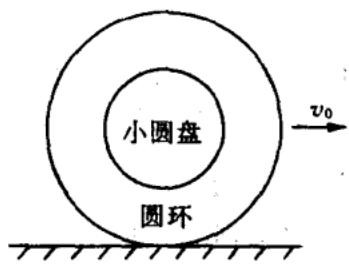
\includegraphics[width=0.3\textwidth]{figures/图5_75.jpg}
\end{center}

\vfill

\newpage

\textbf{5-54} 匀质小球从圆柱面顶端自静止下滚，过程参量均已在图 5-78 中示出.
(1) 为保证在 $\phi \leqslant 45^{\circ}$ 的范围内小球作纯滚动，试求摩擦因数 $\mu$ 的取值范围；
(2) 设 $\mu=0.7$ ，试求纯滚结束时小球质心速度 $v_{1}$ ;
(3) 试求小球离开圆柱面时角位置 $\phi$ 所满足的方程(不必求解).

\begin{center}
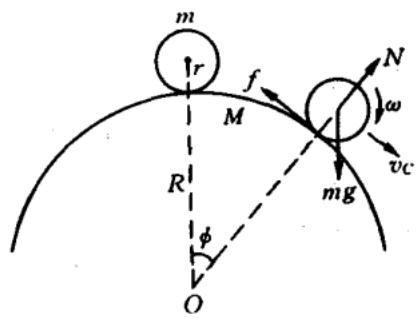
\includegraphics[width=0.3\textwidth]{figures/图5_78.jpg}
\end{center}



\vfill

\textbf{5-55} 质量 $M$ 、半径 $R$ 的匀质圆筒直立地放在光滑水平面上，质量 $m$ 的小球可从圆筒顶部沿圆筒内壁的等距螺旋构槽无摩擦地下滑，筒高 $h$ 恰好等于螺距. 将系统从静止状态自由释放，试求小球落地前相对地面系通过的路程 $s$ .

\begin{center}
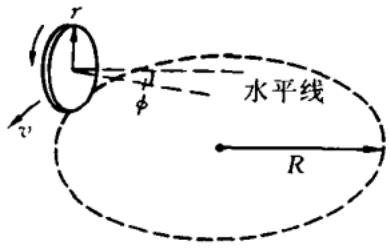
\includegraphics[width=0.3\textwidth]{figures/图5_80.jpg}
\end{center}

\vfill

\newpage

\textbf{5-56} 小心地让一枚硬币在水平桌面上纯滚动，有可能会滚出一个圆周轨道来，此时硬币自转轴稍稍向内倾斜，如图5-80所示.设圆轨道半径为 $R$ ，硬币半径 $r\ll R$ ，硬币中心速度为 $\pmb{v}$ ，试求自转轴小倾角 $\phi$ .

\begin{center}
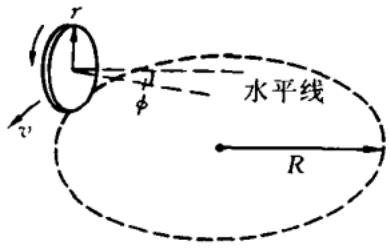
\includegraphics[width=0.3\textwidth]{figures/图5_80.jpg}
\end{center}

\vfill

\newpage

